\documentclass[a4paper, 12bp, twoside]{isee3in1}
%-----------------------------------------------------------------
% global information
%-----------------------------------------------------------------
\newcommand{\StudentName}{钱周越}
\newcommand{\StudentID}{3220104074}
\newcommand{\Supervisor}{李雨文 教授}
\newcommand{\Grade}{2022级}
\newcommand{\Major}{信息与计算科学}
\newcommand{\College}{数学科学学院}
\newcommand{\ProjectName}{基于增量奇异值分解的偏微分方程模型降阶方法}
%-----------------------------------------------------------------
% main doc
%-----------------------------------------------------------------
\begin{document}
% 目录
\makecover
% 正文字体设置
\globalmainfont
% 课题信息页
\newpage
\thispagestyle{infoPage}
\noindent{\setfont{4}{1.5}\selectfont\bfseries {一、题目： \ProjectName}} \\[14bp]
\noindent{\setfont{4}{1.5}\selectfont\bfseries {二、指导老师对文献综述、开题报告、外文翻译的具体要求}}
\vspace{7bp}
\par
% ------ 不要动上面的 ------

文献综述不少于 3000 字，中外文献查阅篇数不少于 8 篇，其中外文文献建议为 3--5 篇。
开题报告不少于 3500 字。
外文翻译译文不少于 3000 字，译文须标注文章标题和原作者姓名，并要求提供外文原文及其出处。
\paragraph*{文献综述要求}
\begin{enumerate}
\item 简述与有限元方法、POD 方法以及缩减基方法（Reduced Basis Method）相关的教材和论文内容，掌握当前该领域的研究基础，并分析毕业论文研究内容与这些文献之间的联系与差异。
\item 分析 POD 方法以及本文拟研究的增量 POD 方法，简要说明这些方法的优缺点，并结合已有文献提出个人思考。
\item 概述所查阅参考文献的主要创新点，并指出其中存在的问题或尚未解决的问题。
\item 从所阅读的外文文献中选择一篇进行完整翻译，要求结构完整、语句通顺，并提供外文原文及其出处。
\end{enumerate}
\paragraph*{开题报告要求}
\begin{enumerate}
\item 简述模型降阶方法以及 POD 方法的应用背景。
\item 在文献综述基础上分析 POD 方法的缺陷，并说明研究增量 POD 方法的必要性。
\item 从理论分析与数值实验两个方面说明选题的可行性。
\item 阐述论文的主要研究内容。
\item 根据研究内容制定具体的实施计划与研究步骤。
\item 明确论文最终预期达到的研究成果。
\end{enumerate}

% ------ 不要动下面的（只改日期即可） ------
\newcommand{\foottext}[1]{{\setfont{-4}{1}\selectfont\bfseries {#1}}}
\vfill
\hfill \makebox[\widthof{\foottext{指导教师（签名）}}][l]{\foottext{指导教师（签名）}}\underline{\makebox[3cm][c]{\foottext{ }}}\par
\vspace{6bp}
\hfill \foottext{2026年3月6日}
\let\foottext\undefined
% 目录页
\newpage
\pagestyle{indexPage}
\tableofcontents
\vspace{12pt}\noindent {\CJKfamily{simhei}\fontsize{12bp}{18bp}\bfseries \hspace{0.36em}《浙江大学本科生文献综述和开题报告考核表》}\vspace{6pt}
% 正文部分
\newpage
\pagestyle{mainPage}
\section{文献综述}

\subsection{研究背景}

偏微分方程模型广泛出现于热传导、渗流、弹性力学、流体力学、电磁散射以及多物理场耦合问题中。在这些应用里，一个极其常见的任务并不是只求解一次方程，而是对同一类模型在不同参数下进行大量重复求解。例如，在参数辨识中需要不断试探候选参数；在最优控制与优化设计中需要反复评估目标函数；在不确定性量化中需要对参数空间进行大量采样；在实时预测与快速决策中又要求每次求解尽可能快。对于这类任务，单次求解的代价固然重要，但更关键的是总体重复求解成本，因此通常被称为 \textbf{many-query 场景}。

以参数化椭圆型方程为例，设
\[
-\nabla\cdot(a(x;\mu)\nabla u(x;\mu)) = f(x),\qquad x\in\Omega,\ \mu\in\mathcal P\subset\mathbb R^p .
\]
经过有限元离散后，可得到大规模线性系统
\[
A(\mu)u_h(\mu)=f(\mu),\qquad A(\mu)\in\mathbb R^{N\times N},\ u_h(\mu)\in\mathbb R^N,\ N\gg 1.
\]
当参数 $\mu$ 改变时，需要反复求解不同的高维线性系统。如果直接对每一个参数点都做一次高精度有限元求解，那么在 many-query 场景下，离散维数 $N$ 与参数样本数 $m$ 的叠加会迅速推高总成本。因此，如何在保证精度的前提下显著降低多参数重复求解开销，成为参数化偏微分方程数值计算中的核心问题 。

正是在这一背景下，\textbf{Reduced Basis（RB）方法} 成为参数化 PDE 的核心降阶技术之一。RB 的基本思想是：大量高维解虽然存在于 $\mathbb R^N$ 中，但对于许多参数化问题，它们往往集中在一个低维流形附近，因此可以用一个维数远小于 $N$ 的低维子空间来逼近 \cite{hesthaven2015,patera_rozza}。若记降阶基矩阵为
\[
V_r\in\mathbb R^{N\times r},\qquad r\ll N,
\]
则可用
\[
u_h(\mu)\approx V_r a(\mu)
\]
来近似高维解，再通过 Galerkin 投影得到降阶系统
\[
V_r^T A(\mu)V_r a(\mu)=V_r^T f(\mu).
\]
这样一来，昂贵的高维求解被转化为低维系统求解。RB 方法最重要的思想之一，就是通过 Offline/Online 分解将主要计算负担集中到离线阶段，而把快速响应留给在线阶段 \cite{hesthaven2015,patera_rozza}。

那么，为什么 RB 往往又要与 SVD 结合？原因在于：RB 的关键并不只是“有一个低维空间”，而是要“构造一个尽可能优的低维空间”。最经典的做法是先收集若干高精度快照
\[
U=[u_h(\mu_1),u_h(\mu_2),\dots,u_h(\mu_m)]\in\mathbb R^{N\times m},
\]
再对快照矩阵做奇异值分解
\[
U=\Phi\Sigma\Psi^T.
\]
取前 $r$ 个左奇异向量便得到 POD 基
\[
V_r=\Phi(:,1:r).
\]
这一步实际上是在 Frobenius 范数意义下寻找对所有快照的最优低秩逼近，因此 POD/SVD 在 RB 中并不是可有可无的附属步骤，而是构造高质量降阶基的核心工具。

进一步的问题是：为什么还要引入 \textbf{增量 SVD}？这是因为在实际的 RB 离线阶段，快照往往并不是一开始就全部拿到的，而是随着参数采样逐步生成的。一方面，贪婪采样、自适应采样等策略都天然带有“迭代新增样本”的结构；另一方面，在大规模仿真中，一次性存储全部快照矩阵本身就可能带来显著的内存压力。因此，若每新加入一个快照都重新对全部快照矩阵做一次 batch SVD，那么计算与存储代价都会很高 。

因此，从 many-query 的整体计算链条看，逻辑是清楚的：many-query 问题需要一个高效的参数化求解框架，因此选择 RB；RB 需要构造尽可能优的低维基，因此自然结合 POD/SVD；而 POD/SVD 在实际离线构基中又面临快照逐步增长、重复分解代价高的问题，因此进一步需要增量 SVD \cite{brand2002,brand2006,zhang2022}。

\subsection{国内外研究进展}

\subsubsection{参数化 PDE 的 Reduced Basis 与 Offline/Online 框架}

参数化 PDE 的模型降阶研究在过去二十余年发展迅速，其中最具代表性的两条主线是 POD 与 RB。Patera、Rozza 以及 Hesthaven 等人的工作系统奠定了参数化方程降阶求解的理论与算法框架：一方面，解流形在适当条件下具有较低的 Kolmogorov 宽度，说明低维近似具有理论可行性；另一方面，Offline/Online 分解将计算量大的部分集中在离线阶段，将快速求解保留到在线阶段，使 many-query 计算成为可能 \cite{patera_rozza,hesthaven2015}。

具体而言，RB 方法的优势在于它并不追求在整个高维空间内逼近，而是针对参数族解的实际分布构造一个问题相关的近似空间。对于许多椭圆型和抛物型问题，参数变化虽然会改变系数矩阵与解向量，但其主导模态常常只占据一个较低维的子空间，因此 RB 可以用很小的 $r$ 达到较高精度。与此同时，若系统具有仿射参数分解，还可以进一步预组装在线阶段的矩阵和向量，从而将在线复杂度降到与 $r$ 而非 $N$ 相关 \cite{hesthaven2015,patera_rozza}。

不过，RB 的瓶颈也非常明确：离线构基。构基质量直接决定在线精度，而构基代价又往往主导整体成本。特别是在样本数较大、单次高精度求解昂贵、快照维数很高时，如何高效地从快照中提取主导信息就成为核心问题。这也是后续 POD/SVD 与增量 SVD 被引入 RB 框架的根本原因 \cite{hesthaven2015,fareed2018}。

\subsubsection{POD/SVD 及其在降阶中的作用}

Proper Orthogonal Decomposition 本质上是一个最优低秩逼近方法。对于快照矩阵
\[
U=[u_1,\dots,u_m]\in\mathbb R^{N\times m},
\]
其截断 SVD
\[
U\approx U_r=\Phi_r\Sigma_r\Psi_r^T
\]
满足
\[
\|U-U_r\|_F^2=\sum_{i>r}\sigma_i^2,
\]
即在所有秩不超过 $r$ 的矩阵中，截断 SVD 给出了最小的 Frobenius 误差。这意味着，如果用前 $r$ 个左奇异向量张成的空间去逼近快照集合，那么从总体均方误差意义看，它是最优的 \cite{golub2013matrix}。

在 PDE 降阶中，POD 有两层意义。第一层是数据压缩：把海量高维快照压缩到少数主模态上。第二层是物理解释：奇异值衰减速度反映了解流形的有效维数，主导模态往往对应主要物理结构。对于 many-query 问题，如果快照在主模态方向上高度集中，那么说明用低维基来代替全维求解具有很强可行性 \cite{hesthaven2015,golub2013matrix}。

然而，经典 POD/SVD 也有天然缺陷。它是典型的 batch 处理方式：需要在构造好全部快照矩阵之后一次性做分解。在离线阶段，这种模式对内存与算力都不友好。特别是在有限元背景下，$N$ 很大，而参数采样数 $m$ 也可能逐步增多，此时反复对大矩阵做完整 SVD 的代价十分显著。

\subsubsection{面向 PDE 数据的加权内积与 core SVD}

对于一般的数据矩阵，标准 Euclidean 内积下的 SVD 已足够。但在有限元离散的 PDE 数据里，更自然的内积通常并不是标准内积，而是由质量矩阵或刚度矩阵诱导的加权内积。例如在有限元空间中，若 $M$ 为质量矩阵，则常考虑
\[
\langle u,v\rangle_W=u^T W v,\qquad W=M.
\]
这意味着正交性、范数与能量贡献的定义都应当相对于 $W$ 而不是单位矩阵。若忽略这一点，所构造的 POD 基就可能与连续问题中的自然能量结构不一致。

为了解决这一问题，Fareed、Singler、Zhang 与 Shen 等人发展了适用于 PDE 仿真数据的 \textbf{incremental POD / core SVD} 框架。在这一框架下，不再简单追求 $Q^TQ=I$，而是要求
\[
Q^T W Q=I,\qquad R^T R=I,
\]
并将
\[
U=Q\Sigma R^T
\]
称为 core SVD。Zhang (2022) 也在文章中沿用了这一定义，并明确指出：若数据来自 Galerkin 型 PDE 仿真，则直接应用标准 Brand 算法会牵涉到 Cholesky 分解，而通过 core SVD 可以更自然地在 weighted inner product 下工作 \cite{fareed2018,zhang2022}。

这一步对基于有限元快照的降阶问题尤其关键，因为研究对象不是一般图像流或机器学习数据，而是有限元离散下的参数化 PDE 快照，因此加权内积框架下的 core SVD 比标准 Euclidean SVD 更符合问题本身的数值结构。

\subsubsection{Brand 增量 SVD 算法及其意义}

增量奇异值分解的核心思想，是在已有矩阵奇异值分解结果的基础上，随着新列向量不断加入，快速更新当前分解，而不必每次都对扩展后的整体矩阵重新执行一次 batch SVD。对于快照逐步生成的 POD/RB 离线阶段，这种“边到达、边更新”的机制尤其重要，因此 Brand 的工作通常被视为增量 SVD 研究中的经典起点 \cite{brand2002,brand2006,zhang2022}。

在有限元离散所诱导的加权内积框架下，设
\[
\langle u,v\rangle_W=u^T W v,
\]
其中 $W$ 通常为质量矩阵或其他对称正定权矩阵。若矩阵 $U_\ell\in\mathbb R^{m\times \ell}$ 的前 $\ell$ 列已经得到了一个截断的 core SVD
\[
U_\ell = Q\Sigma R^T,\qquad Q^T W Q = I,\quad R^T R = I,
\]
其中 $Q\in\mathbb R^{m\times k}$，$\Sigma\in\mathbb R^{k\times k}$，$R\in\mathbb R^{\ell\times k}$，且 $k\le \ell$，那么 Brand 型算法的目标就是在加入新列 $u_{\ell+1}$ 后，快速构造
\[
U_{\ell+1}=[U_\ell,\ u_{\ell+1}]
\]
的更新分解 \cite{brand2002,zhang2022}。

这一算法可以分为“初始化—更新—重正交化”三个层次。

\paragraph{初始化}

若只考虑首个非零列向量 $u_1$，则初始化非常直接。此时
\[
\Sigma = (u_1^T W u_1)^{1/2},\qquad
Q=u_1\Sigma^{-1},\qquad
R=1.
\]
于是便得到单列矩阵 $U_1$ 的初始 core SVD。这个初始化步骤的本质，是先用第一个快照建立一个一维的加权正交基方向，并把对应的尺度信息吸收进奇异值 $\Sigma$ 中 \cite{zhang2022}。

\paragraph{更新}

假设当前已有
\[
U_\ell = Q\Sigma R^T.
\]
当新快照 $u_{\ell+1}$ 到来时，首先将其投影到当前左奇异子空间 $\mathrm{span}(Q)$ 上，并计算残差：
\[
d = Q^T(Wu_{\ell+1}),\qquad
e = u_{\ell+1}-Qd,\qquad
p=(e^TWe)^{1/2}.
\]
这里，$d$ 表示新列在当前基上的坐标，$e$ 表示新信息中无法被现有子空间表示的部分，$p$ 则衡量该残差的加权范数。若 $p>0$，进一步令
\[
\tilde e = e/p.
\]
这样便可写出如下恒等分解：
\[
U_{\ell+1}
=
[Q,\ \tilde e]
\begin{bmatrix}
\Sigma & Q^TWu_{\ell+1}\\
0 & p
\end{bmatrix}
\begin{bmatrix}
R & 0\\
0 & 1
\end{bmatrix}^{T}.
\]
记中间小矩阵为
\[
Y=
\begin{bmatrix}
\Sigma & d\\
0 & p
\end{bmatrix},
\]
则更新问题便被转化为求一个只有 $(k+1)\times(k+1)$ 规模的小矩阵 $Y$ 的 SVD。设
\[
Y = Q_Y\Sigma_Y R_Y^T,
\]
则理论上就可以更新得到
\[
Q^+=[Q,\ \tilde e]Q_Y,\qquad
\Sigma^+=\Sigma_Y,\qquad
R^+=
\begin{bmatrix}
R & 0\\
0 & 1
\end{bmatrix}R_Y.
\]
这正是 Brand 型增量更新的核心：把对大矩阵 $U_{\ell+1}$ 的重新分解，等价转化成对一个低维边界矩阵 $Y$ 的分解，因此显著降低了更新代价 \cite{brand2002,zhang2022}。

\paragraph{截断策略}

在实际应用中，增量 SVD 往往并不追求完整秩，而更关注主导模态，因此需要配合截断机制。Brand 型算法中至少存在两类自然截断：

第一类是\textbf{残差截断}。如果
\[
p<\mathrm{tol},
\]
说明新快照 $u_{\ell+1}$ 与已有子空间非常接近，此时可近似认为 $p=0$、$\tilde e=0$，即新增样本并未真正带来新的独立方向。于是只需更新已有模态，不必增加秩。此时常写成
\[
Q \leftarrow QQ_Y(1\!:\!k,1\!:\!k),\qquad
\Sigma \leftarrow \Sigma_Y(1\!:\!k,1\!:\!k),
\]
\[
R \leftarrow
\begin{bmatrix}
R & 0\\
0 & 1
\end{bmatrix}
R_Y(:,1\!:\!k).
\]

第二类是\textbf{奇异值截断}。若更新后最后若干个奇异值小于给定阈值，则可将其丢弃，仅保留前 $r$ 个主导模态，以控制秩增长并抑制机器精度附近的伪小奇异值。这一策略在面向 PDE 快照的实际 POD/RB 构基中尤其重要，因为目标往往是稳定提取低维主子空间，而不是恢复所有数值上微弱的方向 \cite{fareed2018,fareed2020,zhang2022}。

\paragraph{整体算法结构}

综合来看，Brand 型增量 SVD 的“完全增量版”可以概括为如下流程：先用首列初始化当前分解；随后对每一个新到达的列向量执行更新；每一步更新后，再根据需要进行重正交化修正。其结构可以形式化地写成：
先取 $u_1$ 建立初始的 $(Q,\Sigma,R)$；然后对 $\ell=2,\dots,n$，依次读入 $u_\ell$，执行更新，再执行重正交化，最终返回更新后的三元组 $(Q,\Sigma,R)$ \cite{brand2002,brand2006,zhang2022}。

从 RB/POD 离线构基的角度看，这一算法的重要意义在于：它使得快照矩阵可以按列流式到达，而低维基空间可以同步更新，从而避免“每来一个快照就重做一次 batch SVD”的高额代价。因此，在 many-query 场景下，它不仅是一个数值线性代数技巧，更是连接“高精度快照生成”和“低维缩减基提取”的关键中间环节。

\subsubsection{Brand 2006 及后续改进：从直接更新到间接更新}

尽管上述直接更新形式已经大幅优于反复执行整体 SVD，但如果每一步都显式构造
\[
Q^+=[Q,\tilde e]Q_Y,\qquad
R^+=
\begin{bmatrix}
R & 0\\
0 & 1
\end{bmatrix}R_Y,
\]
那么随着样本数不断增长，左右奇异向量矩阵仍会越来越大，更新成本也会逐步上升。Brand 在后续工作中进一步关注低秩修改问题，试图减少对外层大矩阵的频繁操作，把更多更新压缩到低维空间内部完成 \cite{brand2006}。

沿着这一思路，后续研究逐渐发展出一种更细致的分层结构：将奇异向量更新拆成“大外层矩阵 + 小正交因子”的乘积形式。这样，大矩阵主要负责记录当前子空间的外壳，而频繁发生的旋转与修正则尽可能留在小矩阵内部完成。Zhang (2022) 在此基础上进一步分析了这种结构在 weighted inner product 下的数值行为，并指出：从复杂度角度看，把更新尽量压缩到小矩阵层面是合理的；但从稳定性角度看，必须仔细区分“哪些正交因子容易失去正交性，哪些则相对稳定”，否则算法虽然快，却未必可靠 \cite{zhang2022}。

因此，从 Brand 2002 到 Brand 2006，再到 Zhang 2022，可以看到增量 SVD 的研究主线已经不再只是“如何更新”，而逐渐转向“如何在高效更新的同时维持数值稳定与正交结构”。这也正是该方法从一般数据流处理走向 PDE 降阶构基时必须面对的问题。

\paragraph{增量 POD 的优势与思考}

与传统 batch POD 相比，增量 POD 的首要优势在于其\textbf{更符合快照逐步生成的离线构基过程}。在参数化偏微分方程的 many-query 场景中，高精度快照往往不是一次性全部获得，而是随着参数采样、贪婪选点或自适应策略逐步产生。此时，若每增加一个快照都重新对全部快照矩阵执行一次 batch SVD，则不仅计算代价高，而且要求持续保存全部历史快照，带来较大的存储负担。增量 POD 则可以在已有分解基础上对新到达的数据进行递推更新，使低维基空间随样本增长同步演化，因此在算法结构上更适合实际的离线阶段。

第二，增量 POD 在\textbf{内存占用与可扩展性}方面具有明显优势。对于有限元离散得到的高维快照，状态维数 $N$ 往往很大，而样本数 $m$ 也可能随着参数探索不断增加。传统 batch POD 通常需要保留完整快照矩阵 $U\in\mathbb R^{N\times m}$，当 $N$ 和 $m$ 同时较大时，存储压力会迅速增大。相比之下，增量 POD 只需维护当前的低秩分解结果及少量新增信息，而不必始终回看全部历史数据，因此更适合大规模、流式或长期累积的数据环境。

第三，增量 POD 更有利于\textbf{与参数采样策略和在线构基过程耦合}。在实际 reduced basis 方法中，快照的选取通常并非固定不变，而是与误差估计、贪婪算法、自适应加点等策略紧密相关。增量 POD 的递推更新机制使得“新增一个参数样本—更新一次缩减基”这一过程变得自然可行，从而更容易嵌入完整的 RB 离线流程。这说明增量 POD 的意义并不只是“把 SVD 算得更快”，而是在 many-query 框架下提供了一种更加灵活的基空间构造方式。

当然，增量 POD 的优势并不是无条件的。与 batch POD 相比，它最大的代价在于\textbf{数值稳定性问题更加突出}。由于更新过程是逐步递推的，舍入误差会在多次迭代后不断累积，进而导致正交性退化、奇异值扰动以及截断误差传播等问题；在有限元加权内积框架下，这一问题又会进一步加剧。因此，增量 POD 的真正关键不只是“增量更新”本身，而在于如何在更新效率与数值稳定性之间取得平衡。换言之，增量 POD 的研究重点应当从“能否递推更新”进一步转向“如何稳定地递推更新”。


\subsection{存在问题}

\subsubsection{batch SVD 的重复分解与存储开销}

首先，最直接的问题来自 batch SVD 本身。对于一个 $N\times m$ 的快照矩阵，一次完整分解就已不便宜；若在离线阶段每新增一个快照都重做一次分解，总成本会随样本数迅速增长。更重要的是，batch SVD 通常要求同时保存全部快照数据，这在高维有限元场景下意味着明显的内存压力。因此，对于快照逐步生成的 RB 离线阶段而言，batch SVD 在计算模式上并不理想 \cite{brand2002,brand2006,fareed2018}。

\subsubsection{Brand 增量 SVD 的正交性退化问题}

相比 batch SVD，Brand 型增量 SVD 的最大优势在于每一步更新代价低；但它同时也带来了最核心的数值隐患，即\textbf{正交性退化问题}。理论上，如果在精确算术下每一步都满足
\[
Q^T W Q=I,\qquad R^TR=I,
\]
则更新后的分解始终保持正交结构。然而在实际浮点运算中，矩阵乘法、归一化和重复迭代会不断引入舍入误差；当更新次数达到上千甚至上百万次时，这些误差会逐渐积累，使本应正交的向量组偏离正交条件 \cite{brand2006,zhang2022}。

这一问题之所以严重，是因为它会直接破坏增量 SVD 的数学含义。首先，一旦
\[
Q^T W Q\neq I,
\]
当前分解就不再是严格意义上的 core SVD，相应奇异值也不再准确反映真实谱结构。这样一来，以奇异值大小为依据的截断策略可能失效。其次，POD/RB 的核心是利用主导模态张成一个高质量低维子空间；若基向量之间已经失去正交性，则不同模态可能发生污染与冗余，从而降低缩减基质量，进一步影响在线阶段的精度与稳定性。最后，在有限元加权内积下，这一问题往往比标准 Euclidean 情形更棘手，因为重正交化必须针对 $W$-内积执行，代价显著增加 \cite{fareed2018,zhang2022}。

Brand 型算法的完整流程中通常都会显式加入一个\textbf{重正交化步骤}。以 weighted Gram--Schmidt 为例，其基本思想是：当检测到正交性误差超过阈值时，依次对当前基向量做加权正交投影与归一化修正，即对第 $i$ 个向量减去其在前面各向量方向上的 $W$-投影，再按 $W$-范数归一化。这个过程理论上可以恢复当前基的加权正交性，但在实践中代价很高，尤其当基维数和更新次数都较大时，重正交步骤可能占据算法的大部分耗时 \cite{zhang2022}。

Zhang (2022) 的数值结果清楚地说明了这一点：在标准内积情形 $W=I$ 下，算法的整体代价尚可接受；但在有限元质量矩阵情形 $W=M$ 下，重正交化几乎成为主要耗时来源。文中甚至专门用
\[
E_W=\|I-Q^TWQ\|
\]
来衡量加权正交误差，并展示了在长时间迭代后，即使实施了重正交，正交性仍可能持续退化 \cite{zhang2022}。这说明问题并不只是“要不要重正交”，而是 Brand 型更新结构本身就会持续制造需要修补的正交性误差。

\subsubsection{Brand 开放问题与 Zhang (2022) 的回答}

Brand 在 2006 年提出了一个非常关键的开放问题：为了保证总体数值精度，到底需要多频繁地执行重正交化？这一问题的难点不在于“理论上可不可以重正交”，而在于：如果一味地频繁重正交，算法效率优势会被大幅削弱；但如果重正交不及时，奇异向量的正交结构又会逐渐崩塌 \cite{brand2006}。

Zhang (2022) 对这一开放问题的回答，并不是简单给出一个固定的“每多少步重正交一次”的经验法则，而是更深入地分析了 Brand 型分层更新结构中不同部分的数值脆弱性。其核心观点是：并不是所有正交因子都会同等程度地失去正交性。小规模内部因子由于维度低、连乘次数有限，往往可以在合理精度下保持稳定；真正容易快速退化的，反而是不断扩展的外层大矩阵。因此，算法设计的重点不应放在对所有小矩阵做无差别重正交，而应集中处理最外层、最脆弱的大尺度正交结构 \cite{zhang2022}。

更具体地说，Zhang 提出应尽量避免反复形成并连乘大量小正交矩阵，而把必要的正交修正集中到新增方向相对于当前大基矩阵的递归加权正交化上。这样做的结果是：一方面保留了增量更新“小矩阵计算为主”的效率优势；另一方面又减少了由长链式正交矩阵乘法带来的正交性侵蚀。这实际上把 Brand 原先的开放问题从“多久重正交一次”转化为“应当对哪一层进行重正交”，从而给出了更具结构性的答案 \cite{zhang2022}。

对于基于有限元快照的 PDE 模型降阶而言，这一点尤其重要。因为在加权内积框架下，重正交不仅昂贵，而且直接关系到 POD/RB 基的物理一致性与数值稳定性。因此，如何把 Brand 型增量更新与更稳健的重正交策略结合起来，正是当前这类课题最自然、也最有价值的研究切入点之一。

\subsection{研究展望}

结合上述研究进展与存在问题，可以看到“基于增量奇异值分解的偏微分方程模型降阶方法”具有清晰而具体的研究空间。未来可从以下几个方向深入展开。

第一，\textbf{在参数化椭圆 PDE 上建立完整的算法验证链条}。这一路径最符合本科毕业论文的工作量与可操作性。可选取典型变系数 Poisson 方程或扩散方程作为模型，先实现高精度 FEM 快照生成，再分别实现 batch SVD 构造的 POD/RB 作为基线，以及 weighted inner product 下的增量 core SVD 作为对照。随后系统比较三类指标：近似误差、正交性指标、计算时间与内存占用 \cite{hesthaven2015,fareed2018,zhang2022}。

第二，\textbf{围绕 weighted inner product 下的数值稳定性展开更细致研究}。有限元背景中的自然内积不是标准内积，因此单纯移植一般数据流领域的增量 SVD 算法并不充分。一个值得重点考察的问题是：不同 $W$-正交化策略对误差、耗时和鲁棒性的影响如何。例如，可比较完全重正交、按阈值触发重正交、仅对新增方向递归正交化等不同策略，并用
\[
E_W=\|I-Q^TWQ\|
\]
作为统一指标衡量正交性保持效果。 \cite{fareed2020,zhang2022}。

第三，\textbf{研究截断策略与基维数控制}。增量 SVD 的价值并不只在“更新快”，还在于能边生成、边截断、边控制秩增长。可重点分析两类阈值：一类是残差阈值 $p<\mathrm{tol}$，用来判断新快照是否基本落在当前子空间中；另一类是最小奇异值阈值 $\sigma_k<\mathrm{tol}$，用来决定是否丢弃弱模态。不同阈值会同时影响误差、基维数、在线效率和正交性，因此值得系统实验比较 \cite{brand2002,fareed2018,zhang2022}。

第四，\textbf{从算法层面探索比 Brand 原始更新更稳健的结构}。这部分未必要提出全新的理论算法，但至少可以在实现和比较层面回答一个非常具体的问题：Brand 直接更新、Brand 间接更新、Zhang 型改进更新，在 PDE 快照数据上谁更适合做 POD/RB 离线构基。由于这一方向同时连接了计算效率、正交性保持与加权内积下的数值稳定性，因此即便论文最终侧重数值比较，也具有明确的方法学意义 \cite{brand2006,zhang2022}。

第五，\textbf{将研究结果进一步连接到更复杂的 many-query 任务}。如果时间允许，可以在论文结尾讨论其向更复杂模型的推广，包括抛物型方程、时变 PDE、非线性降阶，以及更复杂的采样机制如贪婪算法和自适应参数选点。这样做的意义在于说明：增量 SVD 并不只是一个线性代数技巧，而是 many-query 降阶计算链条中的关键中间环节，它直接影响离线构基效率，并最终影响在线快速求解的可行性 \cite{hesthaven2015,patera_rozza,zhang2022}。

综上，基于增量奇异值分解的 PDE 模型降阶方法并不是简单地把 SVD 换成增量 SVD，而是在 many-query、RB、POD、weighted inner product、数值正交性与截断控制之间建立起一套完整的方法链。已有研究表明，增量 SVD 在离线构基效率方面具有明显潜力，但其数值稳定性，尤其是加权内积下的正交性保持问题，仍然是进一步研究的关键所在 \cite{brand2002,brand2006,fareed2018,zhang2022}。


% 参考文献
{
\newpage
\bibliographystyle{gbt7714-numerical}
\phantomsection
\subsection{参考文献}
{\normalfont\CJKfamily{simsun}\zihao{5}\setlength{\baselineskip}{14pt}
\renewcommand{\refname}{\vspace{-\baselineskip}}
\bibliography{refs/01_Review}}
}
\section{开题报告}

\subsection{问题提出的背景}

参数化偏微分方程广泛出现于热传导、扩散、渗流、弹性力学、电磁场以及多物理场耦合等问题中。在许多实际应用里，研究者往往并不满足于对某一个固定参数下的模型求解一次，而是需要针对不同参数反复进行数值求解。例如，在参数识别问题中，需要不断调整候选参数并比较模型输出；在优化设计与最优控制中，需要对多个设计变量下的状态方程进行重复评估；在不确定性量化中，需要对参数空间进行大量采样；在实时预测、快速决策和数字孪生等场景中，则要求在参数变化后尽快给出新的近似解。对于这类问题，关键困难不在于单次求解，而在于总体重复求解成本过高，因此常称为 \textbf{many-query 场景}。

以参数化椭圆型方程为例，考虑
\[
-\nabla\cdot(a(x;\mu)\nabla u(x;\mu))=f(x),\qquad x\in\Omega,\ \mu\in\mathcal P\subset\mathbb R^p,
\]
配以适当边界条件。经过有限元离散后，可得到大规模代数系统
\[
A(\mu)u_h(\mu)=f(\mu),\qquad A(\mu)\in\mathbb R^{N\times N},\ u_h(\mu)\in\mathbb R^N,
\]
其中 $N$ 为离散自由度数，通常远大于 $1$。当参数 $\mu$ 在参数域 $\mathcal P$ 中变化时，如果对每一个参数点都独立进行一次高精度有限元求解，那么随着参数样本数的增加，总计算成本将迅速增大。因此，如何在保证近似精度的前提下显著降低重复求解开销，是参数化 PDE 数值计算中的重要问题。

为解决这一问题，模型降阶方法（Model Order Reduction, MOR）得到了广泛研究。其中，\textbf{Reduced Basis（RB）方法} 是参数化 PDE 中最具代表性的降阶框架之一 \cite{hesthaven2015,quarteroni2016,patera_rozza}。其基本思想是：虽然每个高精度解都位于高维空间 $\mathbb R^N$ 中，但对于许多参数化问题，不同参数对应的解往往集中在某个低维流形附近，因此可以构造一个维数远小于 $N$ 的低维子空间来逼近高维解。

若记降阶基矩阵为
\[
V_r\in\mathbb R^{N\times r},\qquad r\ll N,
\]
则可以近似表示
\[
u_h(\mu)\approx V_r a(\mu),
\]
再通过 Galerkin 投影得到低维系统
\[
V_r^T A(\mu)V_r a(\mu)=V_r^T f(\mu).
\]

然而，RB 方法的关键并不只是在于“降维”，更在于如何构造一个尽可能优的低维基空间。最常见的方法是收集若干高精度快照解
\[
U=[u_h(\mu_1),u_h(\mu_2),\dots,u_h(\mu_m)]\in\mathbb R^{N\times m},
\]
并通过奇异值分解
\[
U=\Phi\Sigma\Psi^T
\]
提取前若干个最重要的左奇异向量，作为 POD/RB 基。这种方法在 Frobenius 范数意义下给出最优低秩逼近，因此在模型降阶中具有核心地位 \cite{kunisch2002,trefethen1997}。

进一步的问题是，在 many-query 场景下，快照往往是随着采样过程逐步生成的，而不是一开始就全部获得。如果每增加一个快照都重新对全部快照矩阵做一次 batch SVD，则不仅计算代价高，而且需要较大的存储开销。

基于这一背景，\textbf{增量奇异值分解（incremental SVD）} 成为一个自然且重要的研究方向。Brand 在文献 \cite{brand2002,brand2006} 中提出了经典的增量 SVD 更新方法，可以在新数据到达时更新奇异值分解，而无需重新分解整个矩阵。

\subsubsection{背景介绍}

从数值分析角度看，参数化 PDE 的 many-query 计算具有典型的“离线贵、在线快”的需求结构。RB 方法通常采用 Offline/Online 分解：离线阶段生成快照、构造基空间；在线阶段仅在低维空间内求解，从而大幅减少计算量 \cite{hesthaven2015}。

设快照矩阵为
\[
U=[u_1,u_2,\dots,u_m],
\]
经典方法需要对其统一执行 SVD 分解。而在实际构基中，快照往往逐步生成，因此矩阵具有按列扩展的结构。

在 weighted inner product 下，若
\[
U_\ell = Q\Sigma R^T,\qquad Q^TWQ=I,
\]
则称其为 core SVD。Brand 型增量算法通过将新增快照分解为投影部分和残差部分：

\[
d=Q^T(Wu_{\ell+1}),\qquad
e=u_{\ell+1}-Qd,
\qquad
p=(e^TWe)^{1/2},
\]

从而构造更新矩阵

\[
Y=
\begin{bmatrix}
\Sigma & d\\
0 & p
\end{bmatrix}.
\]

对该小矩阵执行 SVD，即可完成整体更新。

从数学角度看，POD 方法与奇异值分解之间存在紧密联系。
设快照矩阵为
\[
U=[u_1,u_2,\dots,u_m]\in\mathbb R^{N\times m},
\]
其奇异值分解为
\[
U=\Phi\Sigma\Psi^T,
\]
其中 $\Phi$ 和 $\Psi$ 分别为左右奇异向量矩阵，
$\Sigma$ 为奇异值矩阵。
经典结果表明，
取前 $r$ 个左奇异向量所张成的子空间
在 Frobenius 范数意义下
给出了对快照矩阵的最优秩-$r$ 逼近
\cite{trefethen1997}。
因此，
POD 基可以被理解为
快照数据能量最大的主导模态。

然而，
在参数化 PDE 的实际计算中，
快照数量往往不断增加，
如果每一次新增快照都重新执行完整 SVD，
则离线阶段计算成本将迅速增长。
因此，
如何在已有 SVD 基础上进行高效更新，
成为模型降阶中的重要问题。
增量奇异值分解正是在这一背景下提出，
其目标是在新数据到达时更新奇异值分解，
而不必重新处理全部数据。


近年来，增量 POD 方法也被用于 PDE 仿真数据处理中 \cite{fareed2018,fareed2020}。此外，Zhang 在 \cite{zhang2022} 中研究了 weighted inner product 下的增量 SVD 算法，并分析了其数值稳定性。

\subsubsection{POD 方法的局限性与增量 POD 的必要性}
POD 方法由于能够从快照数据中提取主导模态，并在 Frobenius 范数意义下给出最优低秩逼近，因此已成为模型降阶中最常用的构基方法之一。然而，经典 POD 方法通常建立在 \textbf{batch SVD} 的基础上，即必须在收集全部快照之后，对完整快照矩阵一次性执行奇异值分解。这样的处理方式在理论上是清晰的，但在参数化 PDE 的实际计算中存在若干局限性。

首先，\textbf{经典 POD 的计算代价较高}。设快照矩阵为
\[
U=[u_1,u_2,\dots,u_m]\in\mathbb R^{N\times m},
\]
其中 $N$ 是有限元离散后的空间维数，$m$ 是快照数量。在参数化 PDE 的 many-query 场景下，$N$ 往往很大，而 $m$ 也会随着参数采样不断增加。此时，若始终采用 batch SVD，则需要反复对大规模矩阵进行分解，离线阶段的计算成本会迅速升高。尤其当每增加一个新快照都重新对整个快照矩阵做一次 SVD 时，这种重复计算会显著削弱模型降阶在整体流程中的效率优势。

其次，\textbf{经典 POD 对快照存储的要求较高}。batch SVD 通常要求在离线阶段保存全部历史快照，以便统一构造快照矩阵并进行分解。然而，在有限元背景下，每个快照本身就是一个高维向量，当快照数量逐步增加时，存储完整矩阵会带来明显的内存压力。对于大规模参数扫描、长时间仿真或流式生成数据的场景，这一问题尤为突出。

再次，\textbf{经典 POD 不适合快照逐步到达的构基过程}。在实际 reduced basis 方法中，快照往往不是预先全部给定的，而是随着贪婪选点、自适应采样或参数扫描过程逐步生成的。换言之，快照矩阵在离线阶段常常具有“按列不断扩展”的结构。如果仍坚持每次新增样本后都重新执行完整 SVD，则方法在算法结构上与实际数据生成机制并不匹配。因此，经典 POD 更适合静态、一次性的数据处理，而不够适合逐步更新的离线构基过程。

基于以上原因，研究\textbf{增量 POD}方法具有明显必要性。所谓增量 POD，是指在新快照到达时，不必重新处理全部历史数据，而是在已有分解结果的基础上递推更新当前低维基空间。本文中所讨论的增量 POD，主要通过对快照矩阵进行\textbf{增量奇异值分解（incremental SVD）}来实现。其核心思想是：当新的快照列向量加入时，将其分解为相对于当前基空间的投影部分与正交残差部分，再通过一个小规模矩阵的奇异值分解完成整体更新。这样就避免了对整个扩展后快照矩阵重复做 batch SVD。

与经典 POD 相比，增量 POD 主要具有以下几个方面的优势。第一，它能够\textbf{适应快照逐步生成的离线流程}，与参数化 PDE 中常见的贪婪采样、自适应选点等策略更加匹配。第二，它能够\textbf{减少重复分解带来的计算负担}，从而提高离线构基效率。第三，它能够\textbf{降低对完整历史快照存储的依赖}，因而在大规模问题中更具可扩展性。第四，它使得“每增加一个样本就同步更新降阶基”成为可能，从而为更灵活的构基方式提供了算法基础。

当然，增量 POD 并不是对经典 POD 的简单替代。与 batch POD 相比，它虽然在效率和存储方面更具优势，但也带来了新的数值问题。最典型的问题是：在多次递推更新过程中，浮点误差会逐渐积累，导致基向量的正交性退化，进而影响奇异值的准确性、截断策略的可靠性以及最终降阶基的质量。特别是在有限元离散诱导的 weighted inner product 框架下，这一问题会更加明显。因此，增量 POD 的研究重点不仅在于“如何更快地更新”，也在于“如何在更新过程中保持数值稳定性”。

\subsection{论文的主要内容和技术路线}

\subsubsection{主要研究内容}

本文拟以参数化椭圆型偏微分方程为研究对象，围绕“增量奇异值分解在 PDE 模型降阶中的应用”展开研究，主要内容包括以下几个方面。

第一，建立参数化 PDE 模型降阶的基本框架。本文将从参数化椭圆型方程出发，给出其有限元离散形式，并说明在 many-query 场景下直接求解高维系统的成本问题。在此基础上，引入 Reduced Basis 方法和 POD 构基思想，说明快照矩阵的低秩结构为何能够支持模型降阶，以及 SVD 在构造近似最优低维基中的作用。

第二，分析 weighted inner product 下的 core SVD 结构。由于有限元离散通常伴随质量矩阵，因此本文将重点讨论加权内积
\[
\langle u,v\rangle_W=u^TWv
\]
下的正交性与矩阵分解形式，解释为何在 PDE 快照处理中应当考虑 core SVD，而不是简单套用标准 Euclidean SVD。这里的目标不是建立全新的抽象理论，而是在已有定义基础上，准确梳理其与有限元离散和 POD 构基之间的关系。

第三，研究增量 SVD 的初始化与更新机制。设快照矩阵按列逐步生成，本文将分析在已知
\[
U_\ell = Q\Sigma R^T
\]
的条件下，如何通过新增列向量 $u_{\ell+1}$ 构造
\[
U_{\ell+1}=[U_\ell,u_{\ell+1}]
\]
的更新分解。重点包括：投影项与残差项的分离、小规模边界矩阵 $Y$ 的构造、更新后左右奇异向量与奇异值的表达方式，以及当残差很小或新奇异值过小时的截断处理。

第四，讨论重正交与数值稳定性问题。增量 SVD 的主要数值风险在于正交性退化，因此本文将分析为什么浮点误差会导致
\[
Q^TWQ\neq I,
\]
以及这种退化对奇异值真实性、截断可靠性和降阶基质量的影响。在此基础上，讨论加权 Gram--Schmidt 型重正交化的作用及其计算代价，并尝试比较不同策略下的数值表现。

第五，设计数值实验并进行结果比较。本文计划选取一个或若干典型的参数化椭圆型方程作为实验对象，生成有限元快照数据，并分别采用 batch SVD 与增量 core SVD 构造 POD/RB 基。比较指标包括：奇异值衰减、降阶逼近误差、加权正交性误差、离线时间开销以及内存使用情况。通过这些结果，评估增量 SVD 在 PDE 模型降阶中的适用范围与优势。

\subsubsection{技术路线}

本文拟采用“理论梳理—算法实现—数值比较”的技术路线。

第一步，完成文献阅读与问题建模。首先系统阅读参数化 PDE 模型降阶、RB/POD 方法、增量 SVD 以及 weighted inner product 下 core SVD 相关文献，明确课题中的数学对象、算法目标与关键困难。随后选定一个典型的参数化椭圆型方程作为主要测试模型，并确定其边界条件、参数形式和有限元离散方案。

第二步，建立高精度快照生成模块。对选定的参数化 PDE 进行有限元离散，得到高维代数系统
\[
A(\mu)u_h(\mu)=f(\mu).
\]
在给定参数采样集 $\{\mu_1,\dots,\mu_m\}$ 下，计算对应的高精度数值解，并将其组织为快照矩阵
\[
U=[u_h(\mu_1),\dots,u_h(\mu_m)].
\]
同时构造相应的权矩阵 $W$，通常取有限元质量矩阵，以便后续进行 weighted core SVD。

第三步，实现 batch SVD 与增量 SVD 两套离线构基流程。对于 batch 方法，直接对快照矩阵做标准或加权意义下的分解并截断，得到 POD/RB 基；对于增量方法，则按照“初始化—更新—必要时重正交—截断”的流程，逐列处理快照矩阵。这里的重点是保证实现与数学公式一致，并对关键中间量如残差范数 $p$、奇异值阈值和正交性误差进行记录。

第四步，构造降阶模型并进行在线测试。将所得到的低维基代入参数化椭圆方程的离散系统，建立降阶模型
\[
V_r^T A(\mu)V_r a(\mu)=V_r^T f(\mu),
\]
对若干测试参数进行在线求解，并将降阶解与高精度有限元解进行比较，从而评估不同构基方式对在线精度的影响。

第五步，分析实验结果并总结结论。比较 batch SVD 与增量 SVD 在离线时间、内存开销、正交性保持、降阶误差和基维数控制等方面的差异，分析不同截断阈值与重正交策略的影响，并据此总结增量 SVD 在参数化 PDE 模型降阶中的优缺点与适用条件。

\subsubsection{可行性分析}

从研究对象看，本文拟研究的参数化椭圆型方程属于数值分析与科学计算中较为成熟的一类模型，其有限元离散、矩阵组装与数值求解流程较为清晰，适合作为本科阶段模型降阶研究的基础载体。因此，在问题设置上具有较强可行性。

从理论基础看，课题涉及的核心概念包括有限元方法、POD/RB 模型降阶、奇异值分解与 weighted inner product 下的 core SVD。这些内容虽然跨越 PDE 数值、矩阵计算和模型降阶三个方向，但彼此联系紧密，且已有较为清楚的文献基础。本文的目标不是从零建立全新的深层理论，而是在已有理论框架下完成准确梳理、合理实现与数值分析，因此对于本科毕业论文而言是合适的。

从技术实现看，本课题所需的主要计算步骤包括：参数化 PDE 的有限元求解、快照矩阵构造、SVD 或增量 SVD 实现、重正交处理以及降阶误差比较。这些步骤均可借助现有数值计算环境完成，例如 MATLAB、Python 或其他常用科学计算工具。特别是增量 SVD 的更新公式本身由小矩阵 SVD 和向量投影构成，实现难度可控，便于逐步调试和验证。

从工作量看，若将研究重点聚焦在“参数化椭圆方程 + weighted incremental core SVD + 数值比较”这一主线上，则论文内容既有足够的数学深度，又不至于因为问题过大而难以完成。相比试图证明过于复杂的理论结果，这种“数学框架清晰、算法流程完整、实验结果可展示”的选题更符合本科毕业论文的时间与能力边界。

此外，从算法复杂度角度看，
增量 SVD 方法在处理大规模快照矩阵时
具有明显优势。
传统 batch SVD 的计算复杂度通常为
$\mathcal O(Nm^2)$ 或 $\mathcal O(N^2m)$，
当快照维数 $N$ 和样本数量 $m$ 都较大时，
计算成本十分昂贵。
相比之下，
增量 SVD 每次只需要对一个
$(r+1)\times(r+1)$ 的小矩阵执行 SVD，
其计算复杂度显著降低。
因此，
在 many-query 场景下，
采用增量 SVD 构造降阶基
不仅可以减少计算时间，
还可以降低内存存储需求，
从而提高离线阶段的整体效率。

\subsection{研究计划进度安排及预期目标}

\subsubsection{进度安排}

第一阶段：文献调研与问题细化。系统阅读参数化 PDE、Reduced Basis 方法、POD/SVD、incremental SVD 以及 weighted core SVD 相关文献，梳理课题中的基本概念、主要算法与已有结果。在此基础上，明确本文所采用的参数化椭圆方程模型、有限元离散方式以及数值实验平台。

第二阶段：建立高精度模型与快照生成程序。完成参数化椭圆型方程的有限元离散与求解程序，测试不同参数下高精度数值解的正确性与稳定性。随后生成训练快照集与测试快照集，为后续 batch SVD 和增量 SVD 构基提供数据基础。

第三阶段：实现 batch SVD 与增量 core SVD 算法。首先实现标准的快照矩阵分解与 POD 基提取过程，作为比较基线；再实现 weighted inner product 下的增量更新、截断与重正交步骤，并逐步验证更新公式是否正确、正交性是否保持以及截断策略是否有效。

第四阶段：建立降阶模型并开展数值实验。基于两种构基方式得到的低维基，建立参数化椭圆方程的降阶模型，比较其在不同参数点上的近似误差、离线耗时、内存消耗与正交性误差。对实验结果进行整理，并尝试分析不同阈值、不同基维数下的表现差异。

第五阶段：整理结论并撰写论文。对已有理论梳理、算法流程和实验结果进行系统总结，完成文献综述、开题报告、正文初稿与修改稿的撰写，并根据指导教师意见进一步修订，最终形成完整毕业论文。

\subsubsection{预期目标}

第一，较系统地梳理参数化椭圆型 PDE 在 many-query 场景下面临的计算问题，说明 Reduced Basis 方法、POD/SVD 以及增量 SVD 之间的逻辑关系，形成较为清晰的理论背景与问题表述。

第二，在 weighted inner product 框架下，较准确地给出增量 core SVD 的数学描述，包括初始化、更新、截断和重正交等步骤，并解释其在有限元快照数据中的意义。

第三，完成一个可运行的数值实验流程：从高精度有限元快照生成，到 batch SVD 与增量 SVD 构基，再到降阶模型测试与结果比较。通过实验展示增量 SVD 在离线构基中的潜在优势，以及其数值稳定性方面需要关注的问题。

第四，形成一篇结构完整、数学表述准确、实验结果明确的本科毕业论文。论文不追求过度扩张结论，而是力求在选定模型和算法框架下，给出可信、清楚、可复现的分析与比较结果，为后续进一步研究增量 SVD 在更复杂 PDE 模型中的应用打下基础。


% 参考文献
{
\newpage
\bibliographystyle{gbt7714-numerical}
\phantomsection
\subsection{参考文献}
{\normalfont\CJKfamily{simsun}\zihao{5}\setlength{\baselineskip}{14pt}
\renewcommand{\refname}{\vspace{-\baselineskip}}
\bibliography{refs/02_Report}}
}
\section{外文翻译}

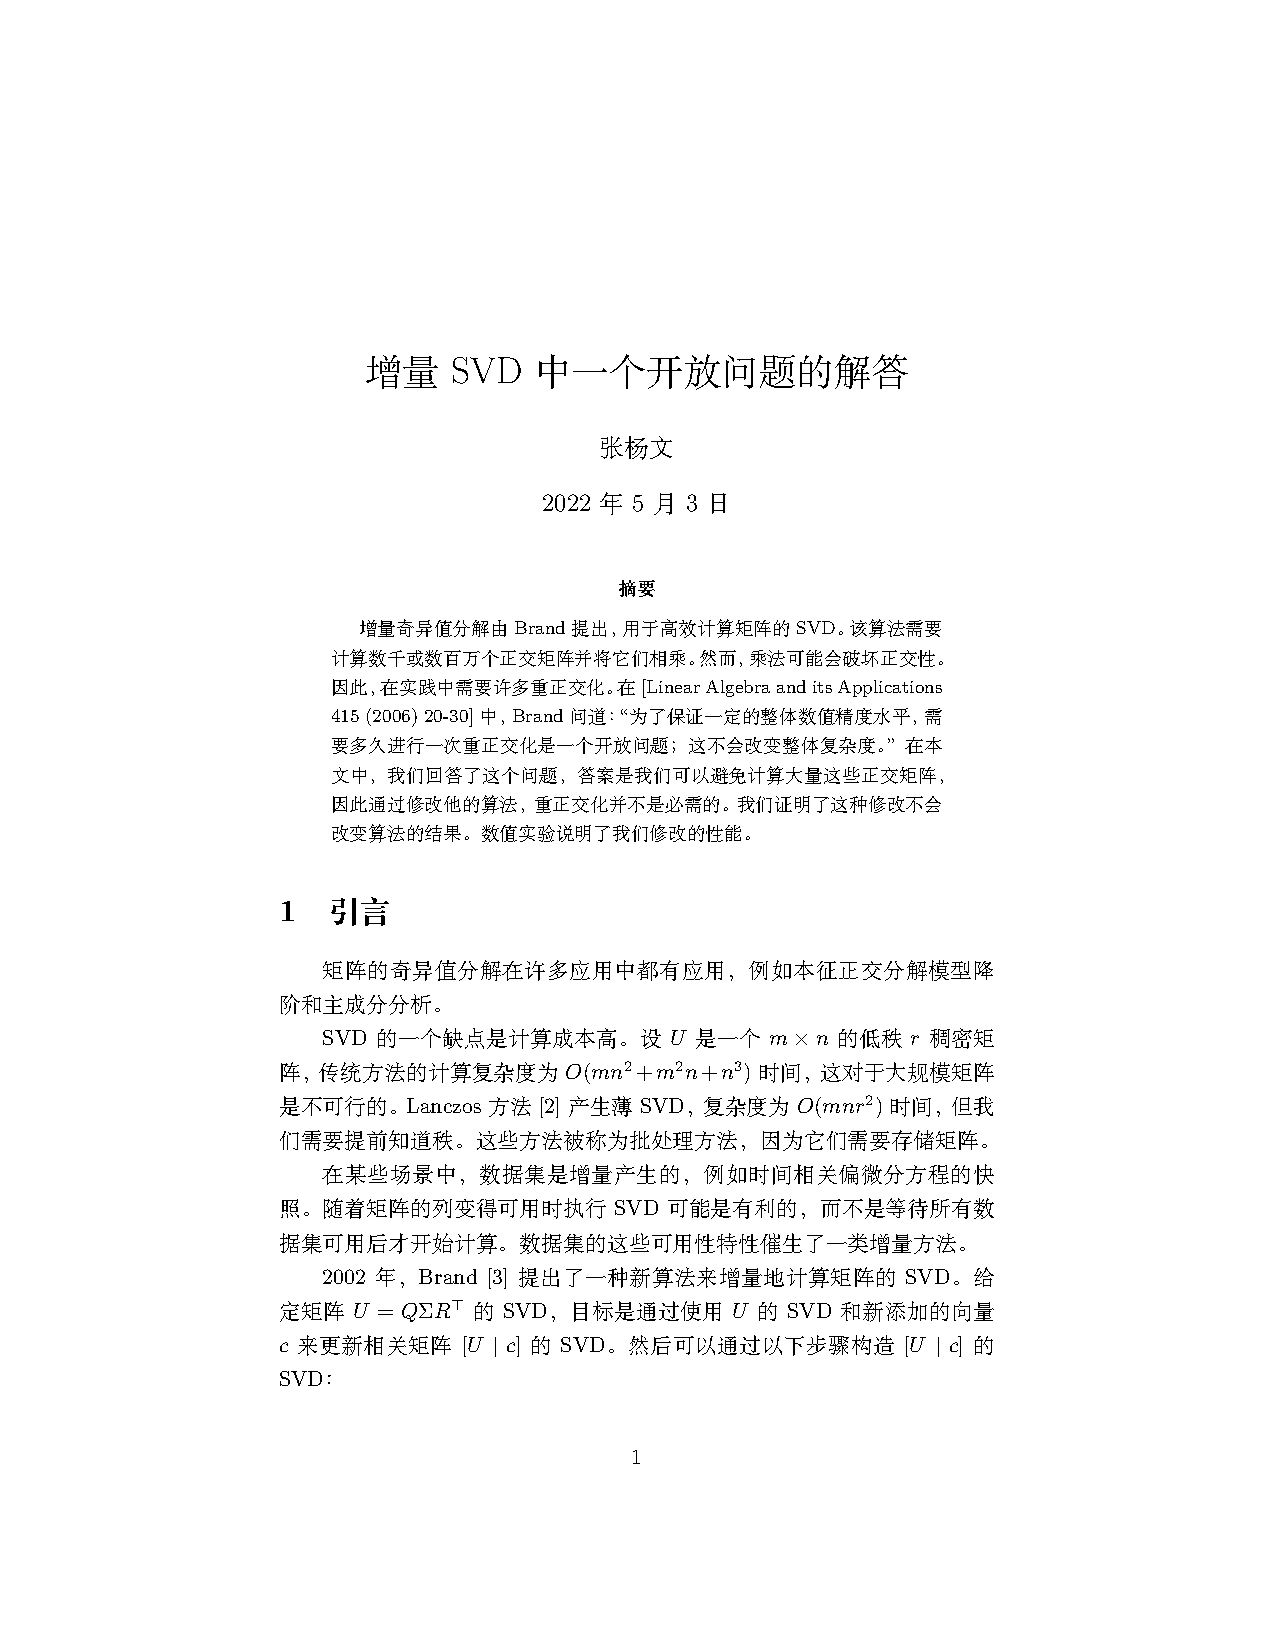
\includepdf[pages=-]{contents/translate.pdf}
\section{外文原文}

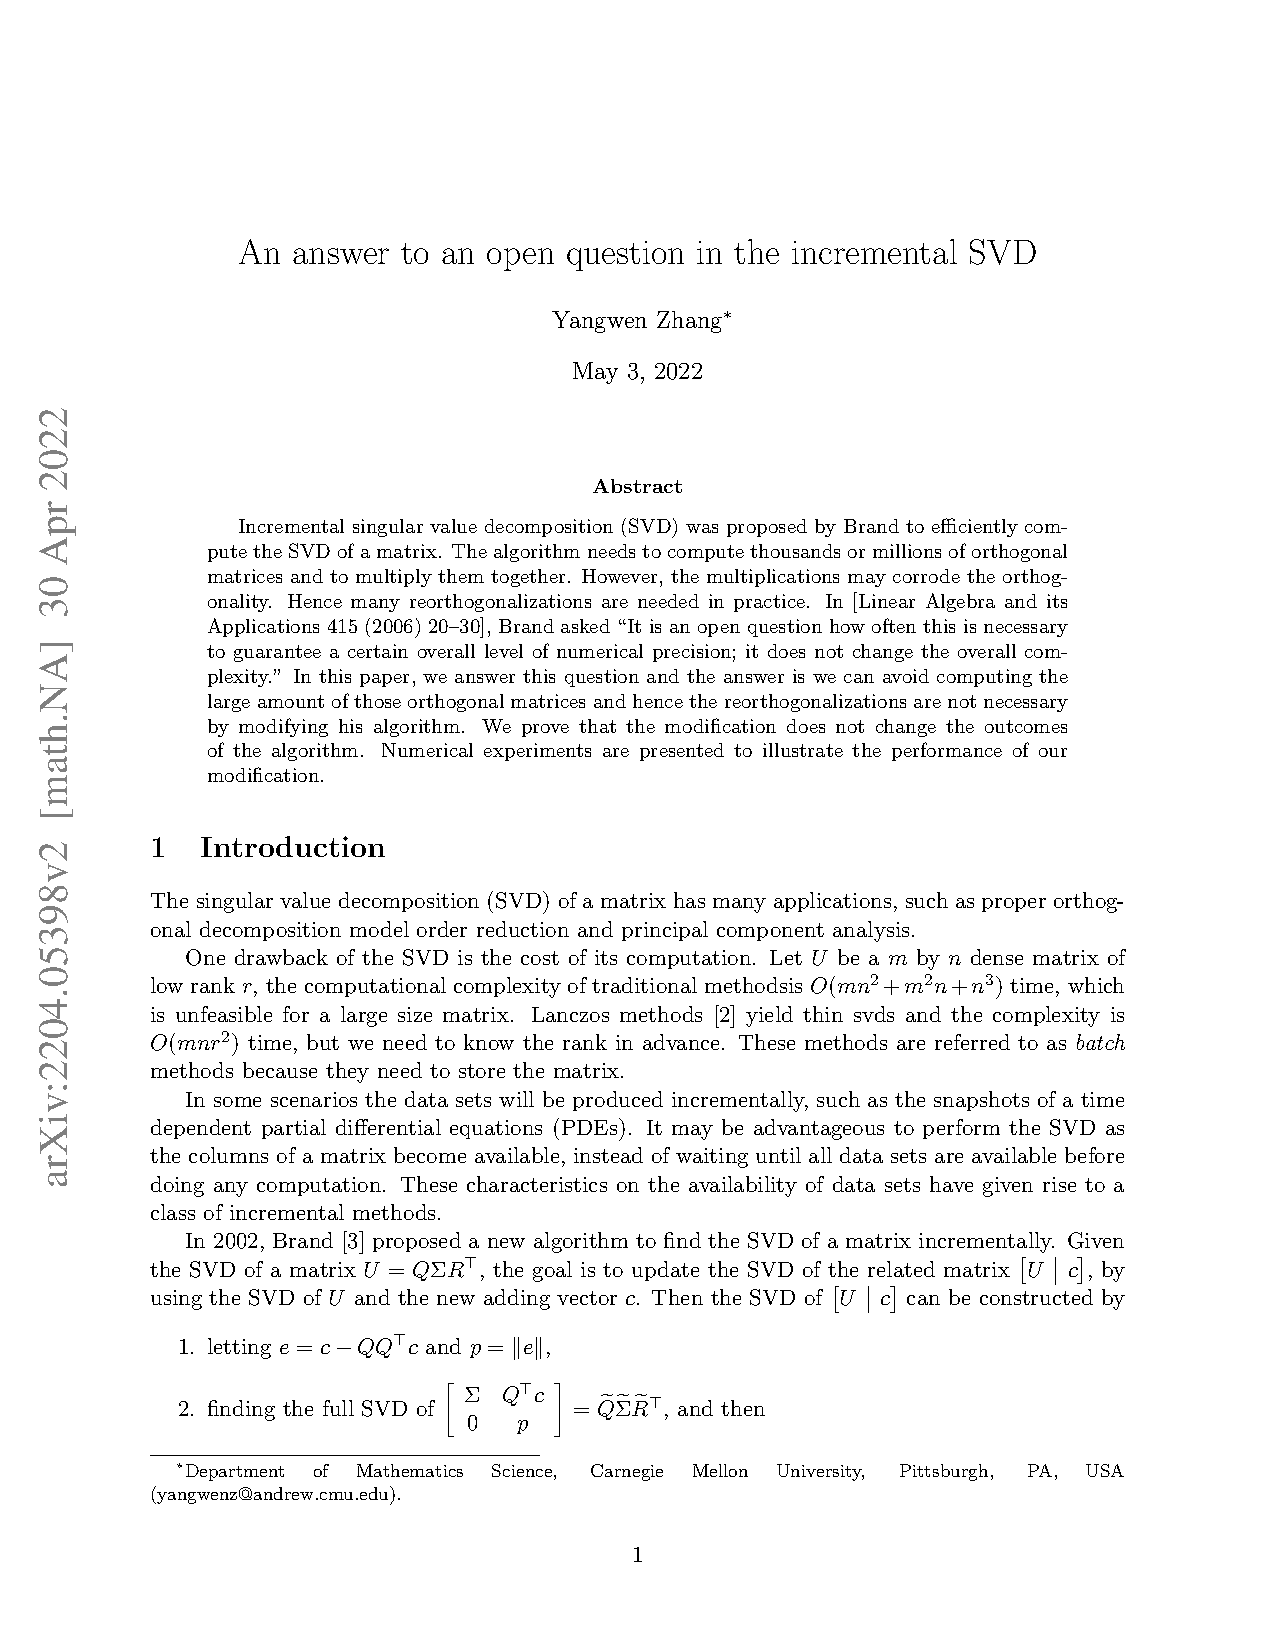
\includepdf[pages=-]{contents/incrementalSVD.pdf}
\pagestyle{empty}\bfseries
\vspace{9bp}
\begin{center}\setfont{-2}{1} 毕业论文（设计）文献综述和开题报告考核\end{center}
\vspace{9bp}
\noindent\setfont{4}{1} 对文献综述、外文翻译和开题报告评语及成绩评定
\vfill


\begin{flushright}
\begin{table}[!htbp]
    \renewcommand{\arraystretch}{2.3}  % 调整行高，可以增大或减小数值
    \hfill
    \begin{tabular}{|>{\centering\arraybackslash}m{3cm}|>{\centering\arraybackslash}m{2.3cm}|>{\centering\arraybackslash}m{2.3cm}|>{\centering\arraybackslash}m{2.3cm}|} \hline
        \bfseries\setfont{4}{1}成绩比例 & \bfseries\setfont{5}{1}文献综述占（10\%） & \bfseries\setfont{5}{1}开题报告占（15\%）& \bfseries\setfont{5}{1}外文翻译占（5\%）\\ \hline
        \bfseries\setfont{4}{1}分值 &  &  & \\ \hline
    \end{tabular}
\end{table}  
\vspace{15bp}
{\hfill {\setfont{-4}{1.5}\bfseries 开题报告答辩小组负责人（签名）\underline{\makebox[3cm]{}}}}\\[6bp]
\hfill {\setfont{-4}{1.5}  2025年\quad\quad  月\quad\quad  日}
\end{flushright} 
\end{document}